\subsection{Camera-Aware Training}
Since Wan2.2-TI2V does not take camera trajectories as input, we first train
the bidirectional model on pose-annotated videos to support explicit 6-DoF
camera control.
% 
Projective Positional Encoding (PRoPE)~\citep{li2025cameras} introduces a relative conditioning mechanism by introducing both inter-camera frustum relationships and camera-agnostic token positions (e.g., RoPE~\citep{su2024roformer}) directly into transformer self-attention blocks.
Mathematically, for a sequence of input tokens $X=\{x_s\}_{s=1}^{S}$, $X\in R^{S\times d}$, $x_s\in R^{d}$, it defines a per-token matrix $D_s^{PRoPE} \in \mathbb{R}^{d \times d}$  composed of two complementary submatrices of shape $\frac{d}{2} \times \frac{d}{2}$:
$$D_s^{PRoPE} = \begin{bmatrix} D_s^{Proj} & 0 \\ 0 & D_s^{RoPE} \end{bmatrix}.$$
The first submatrix, $D_s^{Proj}$, encodes the full projective camera geometry using the world-to-image projection matrix.
The second submatrix, $D_s^{RoPE}$, replicates the standard rotary position embeddings (RoPE). The matrix $D_s^{PRoPE}$ is applied to the attention query and key tokens via matrix multiplication.

Directly applying PRoPE can be expensive on long videos for both training and inference, as it requires adding extra attention modules to the DiT backbone in a layer-wise manner, nearly doubling the overall computational cost.
We argue that PRoPE primarily captures the view-dependent high-level semantics.
Therefore, computing attention over the full-resolution video token set, which contains complete semantics, is unnecessary.
To this end, we introduce a lightweight variant of PRoPE as displayed in Figure~\ref{fig:efficient-prope}. The key idea is to focus on a downsampled set of tokens. Specifically, we downsample the PRoPE attention input tokens $X^{PRoPE}$ along the spatial dimension and project them into a lower-dimensional query/key/value space, yielding
$X^{PRoPE} \in \mathbb{R}^{N \times d'}$ where $d' < d$ and $N$ is the number of downsampled tokens.  This makes camera control highly efficient during both training and inference  while retaining most of the controllability. For example, given a 5-second 720P video, the VAE of Wan2.2 5B maps it to $S=18480$ tokens, while we downsample it to $N=4096$ tokens before computing PRoPE attention, indicating a more than 4.5x spatial downsampling ratio. Consequently, it significantly reduces the training and inference time by approximately 50\% and 30\% respectively.

\begin{wrapfigure}[16]{r}{0.45\textwidth}
    \vspace{-1.0\baselineskip}
    \centering
    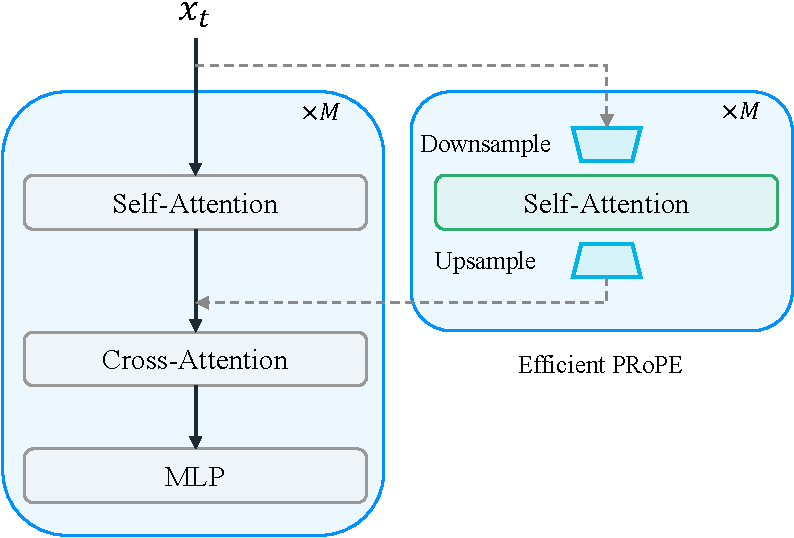
\includegraphics[width=\linewidth]{figures/efficient_prope.pdf}
    \caption{Our Efficient PRoPE (\eprope{}) component is attached to each DiT attention layer. We neglect the adaLN modulation for simplicity.}
    \label{fig:efficient-prope}
\end{wrapfigure}
\paragraph{\bf{Efficient PRoPE (\eprope{}).}}

Additionally, we omit the $D_s^{RoPE}$ component and use only the projective submatrix $D_s^{Proj}$, since the original attention in
the DiT backbone already provides sufficient spatiotemporal inductive bias for fine-grained semantic modeling. After PRoPE attention, we upsample the output tokens back to the original resolution and simply add them to the original DiT attention output. With standard denoising objective, we train PRoPE modules by freezing the DiT backbone and only backpropagating the gradients to the PRoPE parameters.
We compare the performance of PRoPE and \eprope{} in Table~\ref{tab:prope}.

Interestingly, during inference, we empirically find that the downstream model can still leverage the pre-trained PRoPE component in a plug-and-play manner even when trained without it, suggesting the strong and robust geometric bias of PRoPE.

\begin{table}[H]
\caption{Comparing PRoPE and \eprope{} on Omni-WorldBench~\citep{wu2026omniworldbench}. \eprope{} achieves comparable camera control performance to the full PRoPE while being more computationally efficient. Latency is measured as the average time (in seconds) to generate a 5-second video at $1280 \times 720$ resolution on 8 NVIDIA H20 GPUs.}
\label{tab:prope}
\centering
\renewcommand{\arraystretch}{1}
\renewcommand{\tabularxcolumn}[1]{m{#1}}                                  
\footnotesize
\setlength{\tabcolsep}{2.8pt}
\begin{tabularx}{\linewidth}{@{}p{.9in}*{7}{>{\centering\arraybackslash}X}@{}}
% \begin{tabularx}{\linewidth}{l c c c c c c c}
\toprule
\rowcolor{amapblue}
\textcolor{white}{\textbf{Model}} &
\textcolor{white}{\textbf{\shortstack{Camera\\Control $\uparrow$}}} &
\textcolor{white}{\textbf{\shortstack{Image\\Quality $\uparrow$}}} &
\textcolor{white}{\textbf{\shortstack{Dynamic\\Degree $\uparrow$}}} &
\textcolor{white}{\textbf{\shortstack{Transition\\Detect $\uparrow$}}} &
\textcolor{white}{\textbf{\shortstack{Temporal\\Flicker $\uparrow$}}} &
\textcolor{white}{\textbf{\shortstack{Motion\\Smooth. $\uparrow$}}} &
\textcolor{white}{\textbf{\shortstack{Latency $\downarrow$}}} \\
% Model & Camera Control $\uparrow$ & \shortstack{Image\\Quality $\uparrow$} & Dynamic Degree $\uparrow$  & Transition Detect $\uparrow$ & Temporal Flicker $\uparrow$  & Motion Smoothness $\uparrow$ & Inference Latency $\downarrow$ \\
\midrule
\rowcolor{TableRowAlt}
PRoPE & 73.89 & 66.15 & 87.5 & 96.67 & 96.02 & 98.65 & 80 \\
\eprope{} & 73.75 & 66.75 & 85.83 & 98.33 & 96.17 & 98.79 & 59 \\
\bottomrule
\end{tabularx}
\end{table}
